\chapter{Proposed Architecture}
\label{architecture}
\blindtext[3]


\begin{figure}
\centering
  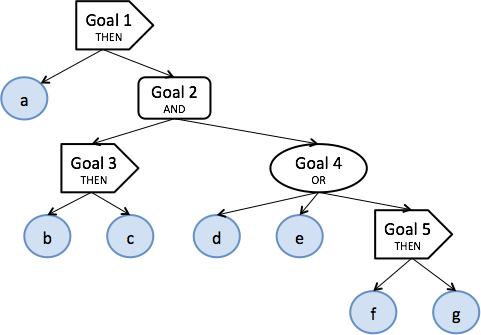
\includegraphics[width=11cm]{task_img}
\caption{Representation of task: a {\bf THEN} ((b {\bf THEN} c) {\bf AND} (d {\bf OR} e {\bf OR} (f {\bf THEN} g))).}
\label{fig:task_representation}
\end{figure}

\blindtext[3]

\section{Update Loop}
\label{sec:updateloop}
\begin{algorithm}
\caption{Behavior update loop}
\label{alg:update}
\begin{algorithmic}[1]
\IF {$Not~Done$}
  \IF {$Is~Active$}
    \IF {$Preconditions$}
      \IF {$BEHAVIOR~NODE$}
      \STATE $Activate:$
        \STATE $~~~Mutex Acquired \Rightarrow state \leftarrow running$
      \ELSIF {$GOAL~NODE$}
        \STATE $Activate:$
          \STATE $~~~state \leftarrow done$
      \ENDIF
    \ELSE
      \STATE $SpreadActivation$
    \ENDIF
    \STATE \emph{ActivationFalloff} $\Rightarrow \alpha ~*$ \emph{activation\_level}  
  \ENDIF
\ENDIF
\end{algorithmic}
\label{update-loop}
\end{algorithm}

\subsection{Activation Potential Spreading}
\blindtext
%%%%%%%%%%%%%%%%%%%%%%%%%%%%%%%%%%%%%%%%%%%%%%%%%%%%%%%%%%%%%%%%%%%%%%%%%%%%%%%%
\begin{figure}
\centering
  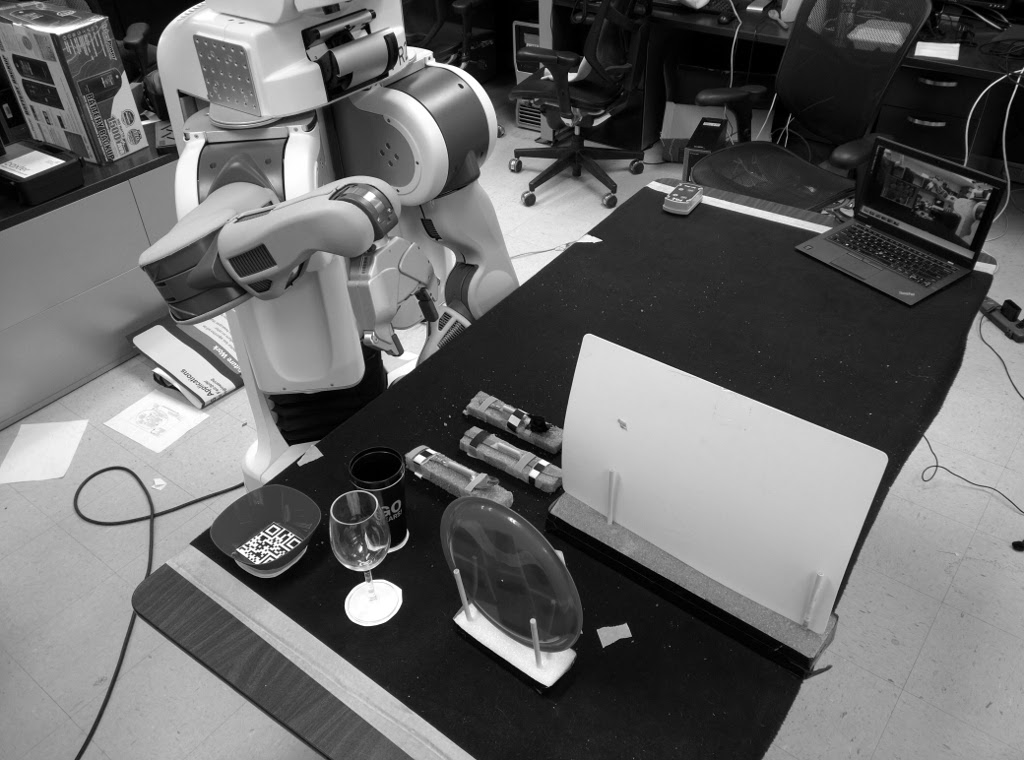
\includegraphics[width=\textwidth]{bw_task_environment}
\caption{Experimental setup.}
\label{fig:setup}       % Give a unique label
\end{figure}
%%%%%%%%%%%%%%%%%%%%%%%%%%%%%%%%%%%%%%%%%%%%%%%%%%%%%%%%%%%%%%%%%%%%%%%%%%%%%%%%
%%%%%%%%%%%%%%%%%%%%%%%%%%%%%%%%%%%%%%%%%%%%%%%%%%%%%%%%%%%%%%%%%%%%%%%%%%%%%%%%

\section{Summary}
\blindtext